\chapter{Methodology}
\section{Methodology}

\hspace*{0.5in}Referring to Fig.3.1 which shows the complete system architecture diagram explaining the overall process flow and component interactions of the proposed Generative AI-based skincare recommendation system, with particular emphasis on the LLM and RAG pipeline modules.

\begin{enumerate}
    \item \textbf{User Registration and Profile Setup:}\\
    The user creates an account through Firebase Authentication. During onboarding, a structured profile form collects skin type (oily, dry, combination, sensitive), age, known allergies, diagnosed hormonal conditions (PCOS, hypothyroidism, menopause), current medications, and lifestyle parameters (sleep quality, stress level, diet type, water intake). This profile is stored in Firebase Realtime Database and retrieved on every subsequent session to provide personalised context to the LLM.

    \item \textbf{Skin Image Upload and Preprocessing:}\\
    The user uploads a facial photograph via the React.js frontend. The image is validated for format (JPEG/PNG), minimum resolution, and approximate facial region coverage. On the FastAPI backend, the image undergoes resizing to 224$\times$224 pixels, pixel normalisation (mean subtraction, std division per channel), and brightness/contrast augmentation for robustness before passing to the detection model.

    \item \textbf{CNN/ViT Skin Condition Classification:}\\
    The preprocessed image is passed through an EfficientNet-B3 CNN backbone for local texture and lesion feature extraction, and simultaneously through a fine-tuned ViT-B/16 for global attention-based feature localisation. The two output probability vectors are fused via late fusion (weighted softmax averaging), producing a final skin condition classification label (e.g., Acne Grade II, Melasma, Rosacea) along with a confidence score and a Grad-CAM heatmap for explainability.

    \item \textbf{Prompt Construction:}\\
    A structured prompt builder on the FastAPI backend assembles the following inputs:
    \begin{itemize}
        \item The skin condition label and severity score from the CNN/ViT model
        \item The user's hormonal profile and relevant medical history from Firebase
        \item The top-$k$ retrieved knowledge chunks from the RAG pipeline
    \end{itemize}
    The prompt follows a structured template designed to elicit a well-formatted, hormone-aware recommendation, as informed by the prompt engineering principles of Kocbek et al. (2025).

    \item \textbf{RAG Knowledge Retrieval (LangChain):}\\
    The combined query — condition label plus hormonal context — is embedded using a SentenceTransformer model (all-MiniLM-L6-v2). The embedding is used to perform a top-$k$ similarity search against a FAISS vector store indexed with dermatological literature, ingredient safety databases, and clinical guidelines. Retrieved document chunks are ranked by cosine similarity score and the top 5 are passed to the prompt builder.

    \item \textbf{LLM Recommendation Generation (Claude / GPT-4):}\\
    The assembled prompt is submitted to the Claude or GPT-4 API. The LLM synthesises all inputs — detection output, hormonal context, user profile, and retrieved evidence — to generate a comprehensive skincare plan structured as:
    \begin{itemize}[label=$\diamond$]
        \item Morning and evening skincare routine (step-by-step with product type and key ingredients)
        \item Ingredient-level recommendations and contraindications (e.g., niacinamide for PCOS acne; avoid retinoids if pregnant)
        \item Dietary guidance specific to the detected condition and hormonal phase
        \item Follow-up monitoring timeline and red-flag indicators for professional referral
    \end{itemize}
    The response is returned as structured JSON for rendering on the frontend dashboard.

    \item \textbf{LLM Chatbot for Follow-up Queries:}\\
    A LangChain ConversationalRetrievalChain with persistent memory enables the user to ask follow-up questions (e.g., ``Can I use salicylic acid if I have PCOS?'') that are answered with full conversational context and grounded in the same RAG knowledge base.
\end{enumerate}

\begin{figure}[H]
\centering
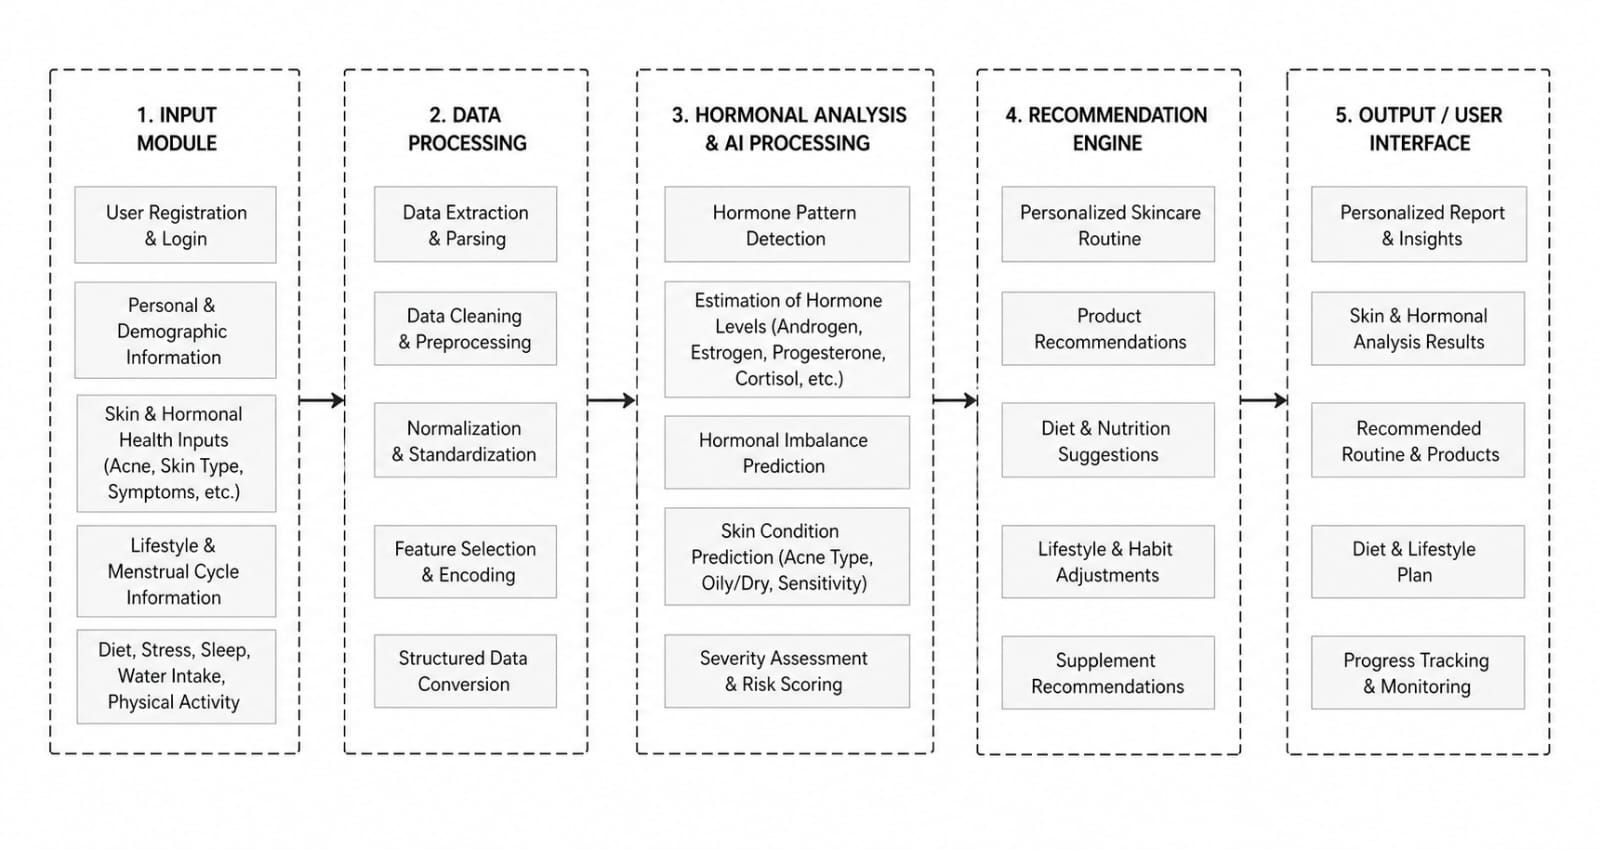
\includegraphics[width=\textwidth]{ATEE_Block.jpeg}
\caption{Hormonal Skincare -- Research-Based Architecture}
\label{gsa1}
\end{figure}


\newpage

\begin{itemize}
    \vspace{2in}
    \item \textbf{\fontsize{15}{12} \selectfont RAG-Powered LLM Recommendation Pipeline}
\end{itemize}
\vspace{0.5cm}
\hspace*{0.5in}Referring to Fig.~\ref{fig:pipeline} which shows the detailed end-to-end flow of the RAG-powered LLM recommendation pipeline — from raw user query to the final structured skincare plan output.\\

\begin{figure}[p]
\centering
\includegraphics[width=\linewidth, height=0.5\textheight, keepaspectratio]{./Atee_pipeline.png}
\caption{RAG-Powered LLM Recommendation Pipeline}
\label{fig:pipeline}
\end{figure}

\hspace*{0.5in}The RAG-LLM pipeline is the core individual contribution of this report. It ensures that every recommendation generated by the LLM is traceable to peer-reviewed dermatological evidence. The pipeline steps are described below:\\

\begin{enumerate}
    \item \textbf{User Query Formation}
    \begin{itemize}
        \item The query comprises three elements: the skin condition classification output, the user's hormonal profile data, and any additional user-entered symptoms or concerns.
        \item These three elements are concatenated into a structured natural language query string by the Prompt Builder module.
    \end{itemize}
    \vspace{0.3cm}

    \item \textbf{Input Preprocessing and Validation}
    \begin{itemize}
        \item The query string is sanitised (removal of PII for logging purposes), validated for completeness, and truncated to fit within the embedding model's maximum token limit.
        \item If mandatory fields are missing (e.g., no hormonal condition specified), a default ``unknown hormonal context'' flag is set and the LLM prompt is adjusted accordingly.
    \end{itemize}
    \vspace{0.3cm}

    \item \textbf{Query Embedding}
    \begin{itemize}
        \item The query string is passed through the SentenceTransformer model (all-MiniLM-L6-v2) to produce a dense 384-dimensional vector embedding.
        \item This embedding captures the semantic meaning of the query for similarity-based retrieval.
    \end{itemize}
    \vspace{0.3cm}

    \item \textbf{Vector Search and Retrieval (FAISS)}
    \begin{itemize}
        \item The query embedding is compared against all document embeddings in the FAISS index using cosine similarity.
        \item The top-5 most similar document chunks are retrieved. Documents are drawn from a curated corpus of dermatological research papers, skincare ingredient safety databases, and clinical practice guidelines.
    \end{itemize}
    \vspace{0.3cm}

    \item \textbf{Prompt Construction}
    \begin{itemize}
        \item Retrieved chunks are injected into a structured system prompt template alongside the condition label, hormonal profile, and user metadata.
        \item The prompt explicitly instructs the LLM to cite the retrieved evidence in its response and to clearly distinguish between established clinical advice and general guidance.
    \end{itemize}
    \vspace{0.3cm}

    \item \textbf{LLM Inference (Claude / GPT-4 API)}
    \begin{itemize}
        \item The assembled prompt is submitted to the LLM API with a temperature of 0.3 (low variance for medical reliability) and a maximum token limit appropriate for a comprehensive skincare plan.
        \item The API response is parsed from JSON, validated for completeness of all expected sections (routine, ingredients, diet, follow-up), and returned to the frontend.
    \end{itemize}
    \vspace{0.3cm}

    \item \textbf{Output Delivery and Logging}
    \begin{itemize}
        \item The structured recommendation is rendered on the React.js dashboard with expandable sections for each component of the skincare plan.
        \item All inference metadata — query, retrieved chunks, prompt, LLM response — is logged to Firebase for model monitoring and future fine-tuning with human feedback.
        \item Users can provide explicit feedback (thumbs up/down per recommendation section) to enable reinforcement learning from human feedback (RLHF) in subsequent model iterations.
    \end{itemize}
\end{enumerate}
